\documentclass[a4paper]{article}
\usepackage[T1]{fontenc}
\usepackage[utf8]{inputenc}
\usepackage{Sweave}
\usepackage{url}
\DefineVerbatimEnvironment{Sinput}{Verbatim} {xleftmargin=2em}
\DefineVerbatimEnvironment{Soutput}{Verbatim}{xleftmargin=2em}
\DefineVerbatimEnvironment{Scode}{Verbatim}{xleftmargin=2em}
\fvset{listparameters={\setlength{\topsep}{0pt}}}
\renewenvironment{Schunk}{\vspace{\topsep}}{\vspace{\topsep}}

\newcommand{\code}[1]{{\texttt{#1}}}
\newcommand{\pkg}[1]{{\textbf{#1}}}
\newcommand{\proglang}[1]{{\textbf{#1}}}

\setlength{\parskip}{3ex plus 2ex minus 2ex}
%%%%%%%%%%%%%%%%%%%%%%%%%%%%%% User specified LaTeX commands.
\usepackage{siunitx}
\sisetup{per=fraction,fraction=nice, decimalsymbol=comma}
\newunit{\wattpeak}{Wp}
\newunit{\watthour}{Wh}
\newunit{\amperehour}{Ah}

\title{\pkg{solaR}: Solar Radiation and Photovoltaic Systems with \proglang{R}}

\author{Oscar Perpiñán Lamigueiro\\Universidad Politécnica de Madrid}


\begin{document}

\section{Introduction}
\label{sec:introduction}

The  \pkg{solaR} package includes a set of functions to calculate
the solar radiation incident on a photovoltaic generator and simulate the 
performance of several applications of the photovoltaic energy \cite{Perpinan2011}.
This package performs the whole calculation procedure from both \emph{daily} and 
\emph{intradaily} global horizontal irradiation to the final productivity of 
grid connected PV systems and water pumping PV systems. 

The package stands on a set of \code{S4} classes. The core of each
class is a group of slots with yearly, monthly, daily and intradaily
multivariate time series (with the \pkg{zoo} package
\cite{Zeileis.Grothendieck2005}). The classes share a variety of
methods to access the information (for example, \code{as.zooD}
provides a \pkg{zoo} object with the daily multivariate time series of
the corresponding object) and several visualisation methods based on
the \pkg{lattice} \cite{Sarkar2010} and \pkg{latticeExtra}
\cite{Sarkar.Andrews2010} packages. The figure \ref{fig:classes}
shows the classes and their relationships. Each frame contains the
name of the class and its constructor function:

\begin{itemize}
\item \code{Sol}: sun geometry. It is created with \code{calcSol}
  (section \ref{sec:solar_geometry}).
\item \code{Meteo}: meteorological data. It can created with several
  functions: \code{readSIAR}, \code{zoo2Meteo}, etc. (section \ref{sec:meteo})
\item \code{G0}: horizontal irradiation and irradiance (contains
  classes \code{Meteo} and \code{Sol}). It is created with
  \code{calcG0} (section \ref{sec:calcG0}).
\item \code{Gef}: effective irradiation and irradiance (contains class
  \code{G0}). It is created with \code{calcGef} (section \ref{sec:effective}).
\item \code{ProdGCPV}: performance of a Grid Connected Photovoltaic
  System (GCPV) (contains class \code{Gef}). It is created with
  \code{prodGCPV} (section \ref{sec:gcpv}).
\item \code{ProdPVPS}: performance of a Photovoltaic Pumping System
  (contains class \code{Gef}). It is created with \code{prodPVPS}
  (section \ref{sec:pumping}).
\item \code{Shade}: shadows in a GCPV system (contains class
  \code{ProdGCPV}). It is created with \code{optimShd} (section
  \ref{sec:trackers}).
\end{itemize}


Besides, \pkg{solaR} includes a tool for the visual statistical analysis of
the performance of a large PV plant composed of several systems.



\begin{figure}
  \centering
  %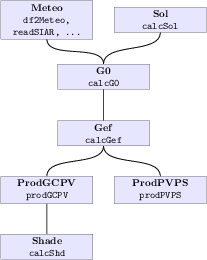
\includegraphics[height=0.4\textheight, keepaspectratio=true]{figs/classScheme}
  \caption{\code{S4} classes and their relationships in the \pkg{solaR} package. Each frame contains the name of the class and its constructor function.}
  \label{fig:classes}
\end{figure}



\section{Solar Geometry}
\label{sec:solar_geometry}
The apparent movement of the Sun is defined with a set of equations
included in the functions \code{fSolD} and
\code{fSolI}. \code{fSolD} computes the daily apparent movement of
the Sun from the Earth. This movement is mainly described (for the
simulation of photovoltaic systems) by the declination angle, the
sunset angle and the daily extra-atmospheric irradiation.  On the
other hand, \code{fSolI} computes the angles which describe the
intradaily apparent movement of the Sun from the Earth.

Besides, the function \code{fBTd} generates time bases with
different structures. For example, the so called
``monthly average days'' (commonly used when only 12 monthly averages
of daily global radiation are available) are obtained with
\code{fBTd(mode = 'prom')}. The azimuth and height solar angles during
these days are displayed in the figure \ref{fig:AzimutAltura}.

\begin{Schunk}
\begin{Sinput}
> lat = 37.2
> SolD <- fSolD(lat, BTd = fBTd(mode = "prom"))
> SolI <- fSolI(SolD, sample = "10 min", keep.night = FALSE)
> mon = month.abb
> p <- xyplot(r2d(AlS) ~ r2d(AzS), groups = month, data = SolI, 
     type = "l", col = "black", 
     xlab = expression(psi[s]), 
     ylab = expression(gamma[s]))
> p + glayer({
     idx <- round(length(x)/2 + 1)
     panel.text(x[idx], y[idx], mon[group.value], pos = 3, offset = 0.2, 
         cex = 0.8)
 })
\end{Sinput}
\end{Schunk}

\begin{figure}
\begin{centering}
%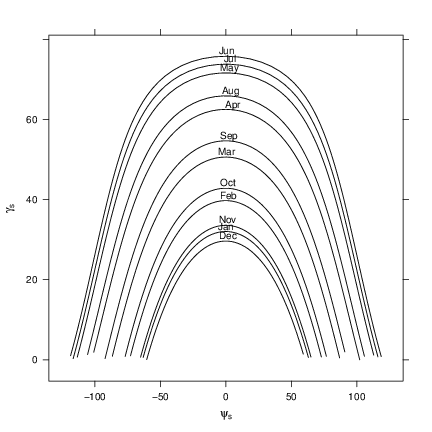
\includegraphics[height=0.4\textheight, keepaspectratio=true]{figs/solaR-006}
\par\end{centering}
\caption{\label{fig:AzimutAltura}Azimuth and height solar angles during the ``average days''.}
\end{figure}


\pkg{solaR} provides four methods for the sun geometry calculations. These
methods are named as 'cooper' \cite{Cooper1969}, 'spencer'
\cite{Spencer1971}, 'michalsky' (default) \cite{Michalsky1988} and
'strous' \cite{Strous2011}:

\begin{Schunk}
\begin{Sinput}
> lat=37.2
> BTd=fBTd(mode='serie')
> solStrous <- fSolD(lat, BTd, method='strous')
> solSpencer <- fSolD(lat, BTd, method='spencer')
> solCooper <- fSolD(lat, BTd, method='cooper')
> solMichalsky <- fSolD(lat, BTd, method='michalsky')
> decDif <- solMichalsky$decl - cbind(solStrous$decl, 
      solSpencer$decl, solCooper$decl)
> names(decDif) <- c('strous', 'spencer', 'cooper')
\end{Sinput}
\end{Schunk}

\begin{figure}
\begin{centering}
%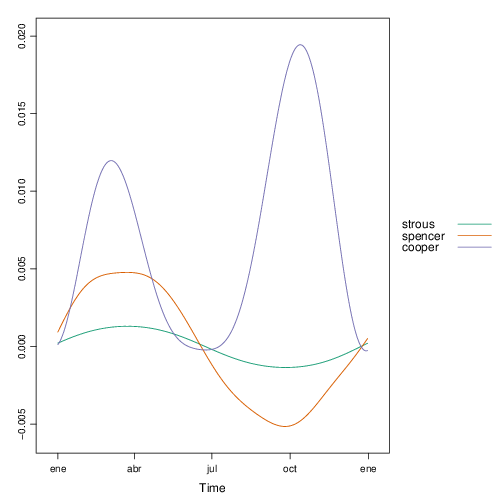
\includegraphics[height=0.4\textheight, keepaspectratio=true]{figs/decl}
\par\end{centering}

\caption{Difference between the \texttt{michalsky} method and others
  to estimate the declination throughout the year\label{fig:Declinacion}}

\end{figure}

These functions are included in a function, \code{calcSol}.
It constructs an object of class \code{Sol} containing in
its slots the \code{zoo} objects created by \code{fSolD} and
\code{fSolI}.  



\section{Solar Radiation}

Values of global horizontal irradiation are commonly available either
as monthly averages of daily values or as a time series of daily
values during one or several years.  The analysis of the performance
of a PV system starts from the transformation of the global horizontal
irradiation to global, diffuse and direct horizontal irradiance and
irradiation, and then irradiance and irradiation on the generator
surface.


\subsection{Irradiation and irradiance on the horizontal plane}
\label{sec:horizontal}
The function \code{fCompD} extracts the diffuse and direct components
from the daily global irradiation on a horizontal surface by means of
regressions between the clearness index and the diffuse fraction
parameters.  This function need the results from \code{fSolD}, a set
of values of global horizontal irradiation
($\si{\watthour\per\meter\squared}$), and the correlation between the
clearness index and the diffuse fraction.  

\pkg{solaR} includes predefined correlations for monthly means of
daily values \cite{Page1961, Liu.Jordan1960}, for daily values
\cite{Collares-Pereira.Rabl1979,Erbs.Klein.ea1982,Miguel.Bilbao.ea2001}
and for intradaily values \cite{Ridley.Boland.ea2010}.  Besides, the
user may define a particular correlation through the argument
\code{f}.

\begin{Schunk}
\begin{Sinput}
> BTd = fBTd(mode = "serie")
> SolD <- fSolD(lat, BTd[100])
> SolI <- fSolI(SolD, sample = "hour")
> G0d = zoo(5000, index(SolD))
> fCompD(SolD, G0d, corr = "Page")
\end{Sinput}
\begin{Soutput}
               Fd    Ktd  G0d  D0d  B0d
2011-04-10 0.4123 0.5201 5000 2062 2938
\end{Soutput}
\begin{Sinput}
> fCompD(SolD, G0d, corr = "CPR")
\end{Sinput}
\begin{Soutput}
               Fd    Ktd  G0d  D0d  B0d
2011-04-10 0.5658 0.5201 5000 2829 2171
\end{Soutput}
\end{Schunk}

The daily profile of the irradiance is obtained with the function
\code{fCompI}.  This function needs the information provided by
\code{fCompD} and \code{fSolI}, or \code{calcSol}. For example,
the profiles for the ``monthly average days'' are obtained with the next code
(fig. \ref{fig:ComponentesIrradiancia}).

\begin{Schunk}
\begin{Sinput}
> sol <- calcSol(lat, fBTd(mode = "prom"), sample = "hour", keep.night = FALSE)
> G0dm = c(2.766, 3.491, 4.494, 5.912, 6.989, 7.742, 7.919, 7.027, 
     5.369, 3.562, 2.814, 2.179) * 1000
> Ta = c(10, 14.1, 15.6, 17.2, 19.3, 21.2, 28.4, 29.9, 24.3, 18.2, 
     17.2, 15.2)
> BD <- readG0dm(G0dm = G0dm, Ta = Ta, lat = 37.2)
> compD <- fCompD(sol, BD, corr = "Page")
> compI <- fCompI(sol, compD)
\end{Sinput}
\end{Schunk}

%
\begin{figure}
\begin{centering}
%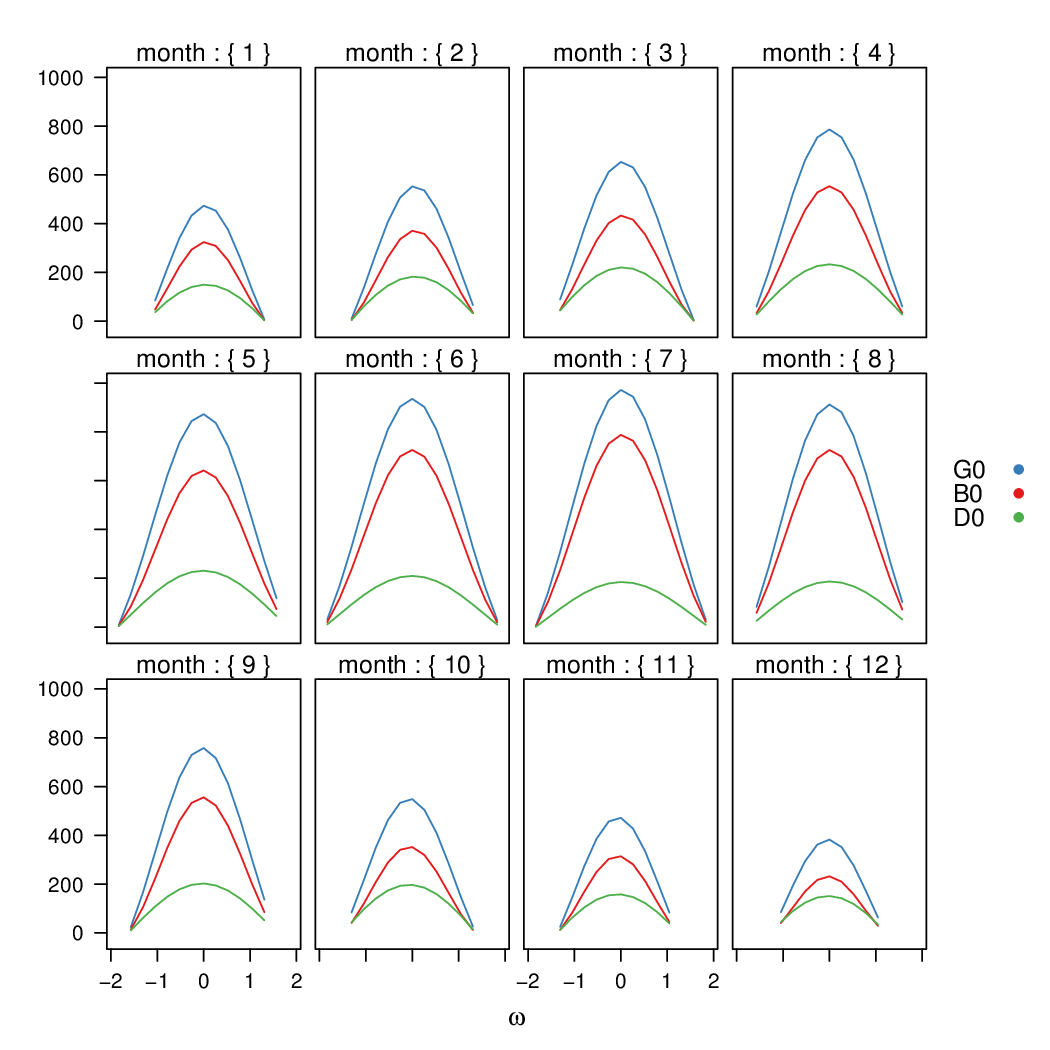
\includegraphics[height=0.4\textheight, keepaspectratio=true]{figs/compI.pdf}
\par\end{centering}
\caption{Global, diffuse, and direct irradiance during the ``monthly average days''.\label{fig:ComponentesIrradiancia}}
\end{figure}

\subsection{Meteorological data}
\label{sec:meteo}
There are several functions to construct a \code{Meteo} object with
radiation and temperature data.  For daily data, the functions
\code{readBD} and \code{df2Meteo} are recommended if it is stored in a
local file or a \code{data.frame}, while \code{readG0dm} is indicated
when only 12 monthly averages are available. The correspondent
functions for intradaily data are \code{readBDi} and
\code{dfI2Meteo}. Besides, \code{zoo2Meteo} can construct a
\code{Meteo} object from a \pkg{zoo} object both for daily and
intradaily data.

For example, the \code{helios} dataset included in the package,
obtained from \url{http://helios.ies-def.upm.es}, can be converted to
a \code{Meteo} object with the next code:
\begin{Schunk}
\begin{Sinput}
> data("helios")
> names(helios) = c("date", "G0", "TempMax", "TempMin")
> bd = df2Meteo(helios, dates.col = "date", lat = 41, source = "helios-IES", 
     format = "%Y/%m/%d")
> bd
\end{Sinput}
\begin{Soutput}
Object of class  Meteo 

Source of meteorological information: bd-helios-IES 
Latitude of source:  41 degrees

Meteorological Data:
     Index                           G0           TempMax         TempMin      
 Min.   :2009-01-01 00:00:00   Min.   :  326   Min.   : 1.41   Min.   :-37.50  
 1st Qu.:2009-04-08 12:00:00   1st Qu.: 2523   1st Qu.:14.41   1st Qu.:  1.95  
 Median :2009-07-07 00:00:00   Median : 4746   Median :23.16   Median :  7.91  
 Mean   :2009-07-04 21:29:54   Mean   : 4812   Mean   :22.59   Mean   :  5.32  
 3rd Qu.:2009-10-03 12:00:00   3rd Qu.: 7140   3rd Qu.:31.06   3rd Qu.: 15.11  
 Max.   :2009-12-31 00:00:00   Max.   :11254   Max.   :38.04   Max.   : 24.80  
\end{Soutput}
\end{Schunk}

On the other hand, the function \code{readSIAR} is able to download
the meteorological data available at \url{www.marm.es/siar}.  This
web page provides daily measurements from a set of agroclimatic
stations located in Spain (figure \ref{fig:siar}). This function needs
the code of the station and its province, and the start and end
date. The codes of stations and provinces are stored at the dataset
\code{SIAR}. 

\begin{figure}
  \centering
%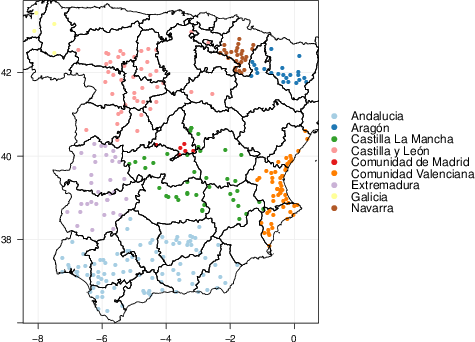
\includegraphics[height=0.45\textheight, keepaspectratio=true]{figs/siar_crop}  
  \caption{Meteorological stations of the SIAR network}
\label{fig:siar}
\end{figure}

\code{readSIAR} constructs an object of class \code{Meteo}. The
raw data is obtained with the method \code{getData}.  If only the
irradiation series is needed, the method \code{getG0} is
recommended. Both methods provide a \pkg{zoo} object. 
For example, the 2009 data from the station at Aranjuez is displayed
in the figure \ref{fig:Aranjuez}.  

\begin{Schunk}
\begin{Sinput}
> Aranjuez <- readSIAR(28, 3, "01/01/2009", "31/12/2009")
> xyplot(G0 ~ TempMedia | month, data = Aranjuez, type = c("p", "r"))
\end{Sinput}
\end{Schunk}

It is important to note that the radiation
measurements available at the web page are in
$\si{\mega\joule\per\meter\squared}$, but \code{readSIAR} converts
the values to $\si{\watthour\per\meter\squared}$:


\begin{figure}
  \centering
%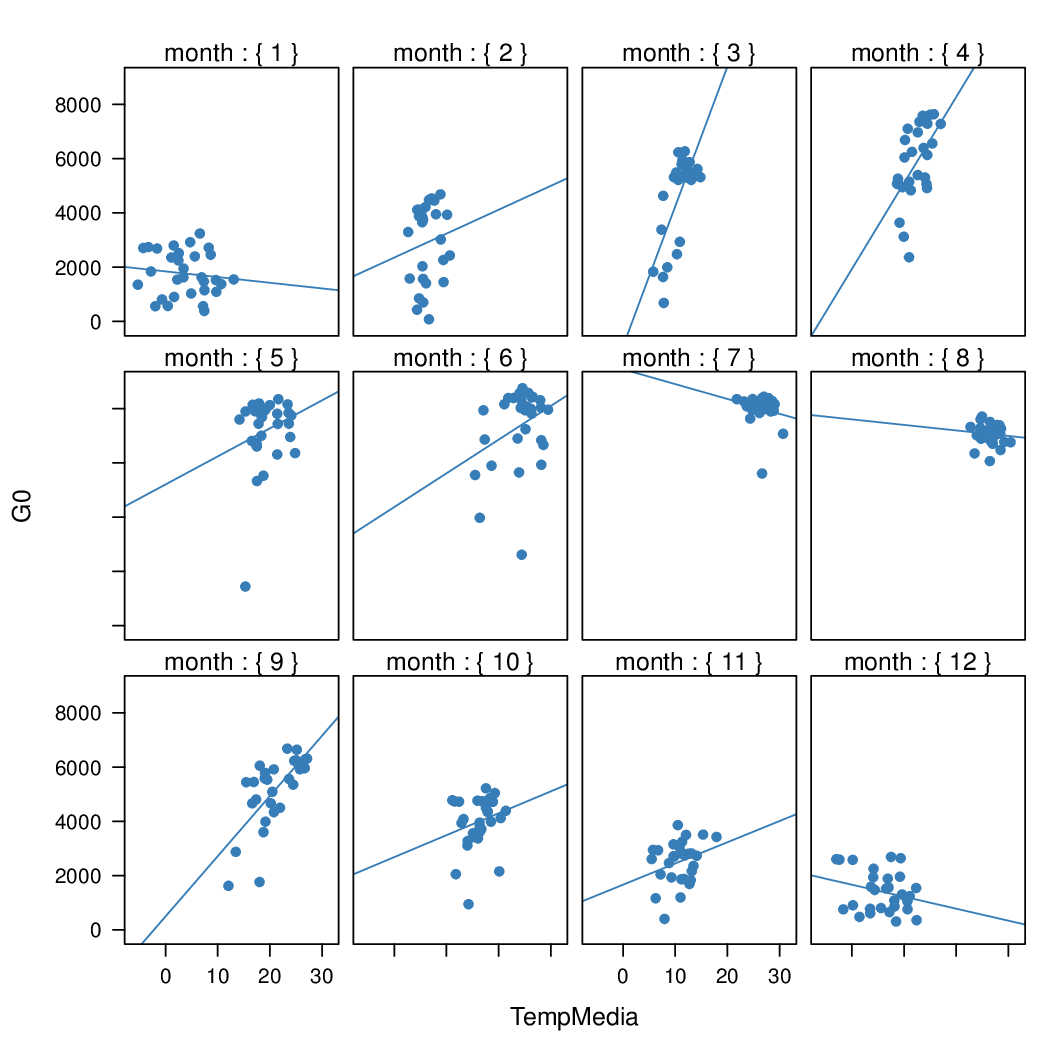
\includegraphics[height=0.4\textheight, keepaspectratio=true]{figs/tempAranjuez.pdf}
  \caption{Daily irradiation and mean temperature in the station of Aranjuez.}
  \label{fig:Aranjuez}
\end{figure}

The SIAR network includes information of maximum and minimum values of
temperature.  The function \code{fTemp} calculates a profile of the
ambient temperature with this information following the method
proposed in \cite{Huld.Suri.ea2006}.  The evolution of this synthetic
time series of temperature during March is displayed in the figure \ref{fig:Ta}.

\begin{Schunk}
\begin{Sinput}
> lat = 41
> sol = calcSol(lat, BTd = indexD(Aranjuez), sample = "hour")
> Temp <- fTemp(sol, Aranjuez)
> wTemp = window(Temp, start = as.POSIXct("2009-03-01"), 
      end = as.POSIXct("2009-03-31"))
> xyplot(wTemp, col = "black", ylab = "T") + 
      layer_(panel.xblocks(x, DoY, col = c("lightgray", "white")))
\end{Sinput}
\end{Schunk}

%
\begin{figure}
\begin{centering}
%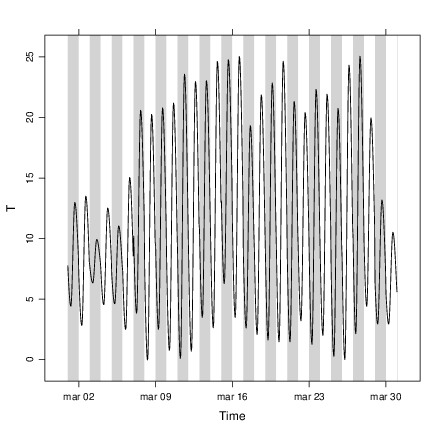
\includegraphics[height=0.4\textheight, keepaspectratio=true]{figs/solaR-020}
\par\end{centering}
\caption{Evolution of the ambient temperature during March 2009 in Aranjuez.\label{fig:Ta}}
\end{figure}



\subsection[The function calcG0]{The function \code{calcG0}}
\label{sec:calcG0}
The previous steps are included in the function \code{calcG0}, the
constructor of the class \code{G0}. For example, with the next code,
the components of horizontal irradiation and irradiance are obtained
from the measurements of the meteorological station of Aranjuez
(figure \ref{fig:calcG0}).

\begin{Schunk}
\begin{Sinput}
> g0 <- calcG0(lat = 37.2, modeRad = "siar", dataRad = list(prov = 28, 
     est = 3, start = "01/01/2009", end = "31/12/2009"))
\end{Sinput}
\end{Schunk}

%
\begin{figure}
\begin{centering}
%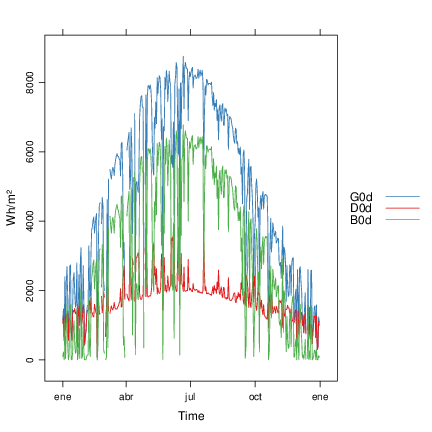
\includegraphics[height=0.4\textheight, keepaspectratio=true]{figs/solaR-022}
% \begin{Schunk}
% \begin{Sinput}
% > xyplot(g0)
% \end{Sinput}
% \end{Schunk}
\par\end{centering}
\caption{Components of horizontal irradiation calculated with \code{calcG0}.\label{fig:calcG0}}
\end{figure}

\pkg{solaR} accepts intradaily irradiation data sources. For example, the \emph{La Ola - Lanai} station at Hawaii
(\url{http://www.nrel.gov/midc/la_ola_lanai/}) from the Measurement and Instrumentation Data Center of the NREL
(NREL-MIDC) provides meteorological data with 1-minute sampling rate\footnote{The data for
  the example are available at
  \url{http://www.nrel.gov/midc/apps/plot.pl?site=LANAI&start=20090722&edy=19&emo=11&eyr=2010&zenloc=19&year=2010&month=11&day=1&endyear=2010&endmonth=11&endday=19&time=1&inst=3&inst=4&inst=5&inst=10&type=data&first=3&math=0&second=-1&value=0.0&global=-1&direct=-1&diffuse=-1&user=0&axis=1}}.  

The local data logger program runs using Greenwich Mean Time (GMT), and
data is converted to Hawaiian Standard Time (HST) after data
collection. The function \code{local2Solar} calculates the Mean Solar
Time of the index. Besides, the horizontal direct irradiation is
obtained, since it is not included in the file.

\begin{Schunk}
\begin{Sinput}
> lat = 20.77
> lon = -156.9339
> dat <- read.zoo(file, 
     col.names = c("date", "hour", "G0", "B", "D0", "Ta"), 
     index = list(1, 2), 
     FUN = function(d, h) as.POSIXct(paste(d, h), 
         format = "%m/%d/%Y %H:%M", tz = "HST"), 
     FUN2 = function(x) local2Solar(x, lon), 
     header = TRUE, sep = ",")
> dat$B0 <- dat$G0 - dat$D0

\end{Sinput}
\end{Schunk}

Finally, the  object \code{Meteo} is obtained with \code{zoo2Meteo} (figure \ref{fig:NREL-MIDC}):

\begin{Schunk}
\begin{Sinput}
> NRELMeteo <- zoo2Meteo(dat, lat = lat, source = "NREL-La Ola-Lanai")
\end{Sinput}
\end{Schunk}

\begin{figure}
  \centering
%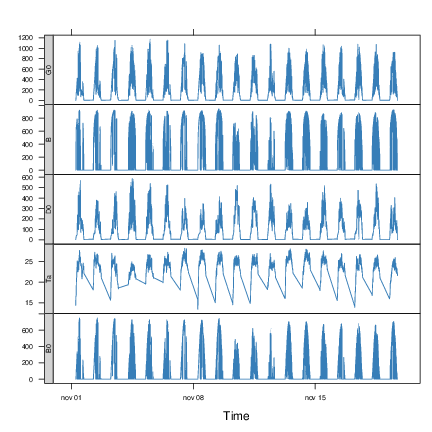
\includegraphics[height=0.4\textheight, keepaspectratio=true]{figs/solaR-025}
  \caption{1-min irradiation data from NREL-MIDC}
  \label{fig:NREL-MIDC}
\end{figure}

With this data, a \code{G0} object can be calculated. Since both
diffuse and direct components are available, no correlation is needed (\code{corr='none'}):

\begin{Schunk}
\begin{Sinput}
> g0NREL <- calcG0(lat = lat, modeRad = "bdI", dataRad = NRELMeteo, 
     corr = "none")
\end{Sinput}
\end{Schunk}

If these components were not available, a fd-kt hourly correlation is
needed \cite{Ridley.Boland.ea2010}:

\begin{Schunk}
\begin{Sinput}
> g0BRL <- calcG0(lat = lat, modeRad = "bdI", dataRad = NRELMeteo, 
     corr = "BRL")
\end{Sinput}
\end{Schunk}

\subsection{Irradiation and irradiance on the generator plane}
\label{sec:effective}

The solar irradiance incident on an inclined surface can be calculated
from the direct and diffuse irradiance on a horizontal surface, and
from the evolution of the angles of the Sun and the surface. The
transformation of the direct radiation is straightforward since only
geometric considerations are needed. However, the treatment of the
diffuse irradiance is more complex since it involves the modelling of
the atmosphere.

There are several models for the estimation of diffuse irradiance on
an inclined surface. The proposal of Hay and McKay combines simplicity
and acceptable results \cite{Hay.McKay1985}. This model divides the
diffuse component in isotropic and anisotropic whose values depends on
a anisotropy index.  

On the other hand, the effective irradiance ---the fraction of the
incident irradiance that reaches the cells inside a PV module--- is
calculated with the losses due to the angle of incidence and
dirtiness. This behaviour can be simulated with a model proposed by
Martin and Ruiz requiring information about the angles of the surface
and the level of dirtiness \cite{Martin.Ruiz2001}.

The orientation, azimuth and incidence angle are calculated from the
results of \code{fSolI} or \code{calcSol} with the functions
\code{fTheta} and \code{fInclin}. These functions can estimate
the geometry and irradiance for fixed systems, and two-axis and
horizontal North-South trackers. Besides, the movement of a horizontal NS
tracker due to the backtracking strategy \cite{Panico.Garvison.ea1991}
can be calculated with information about the tracker and the distance
between the trackers included in the system.

Both functions are integrated in \code{calcGef}, which constructs an
object of class \code{Gef}. 

For example, with the results of section \ref{sec:calcG0}, the
irradiance and irradiation on a fixed surface can be estimated. The figure
\ref{fig:GefG0vsTheta} shows the relation between the effective and
incident irradiance versus the cosine of the angle of incidence for
this system.

\begin{Schunk}
\begin{Sinput}
> gef <- calcGef(lat = 37.2, modeRad = "prev", dataRad = g0, 
      beta = 30)
> xyplot(Gef/G ~ cosTheta | month, data = gef, type = c("p", 
      "smooth"), cex = 0.4, alpha = 0.5)
\end{Sinput}
\end{Schunk}

%
\begin{figure}
\begin{centering}
%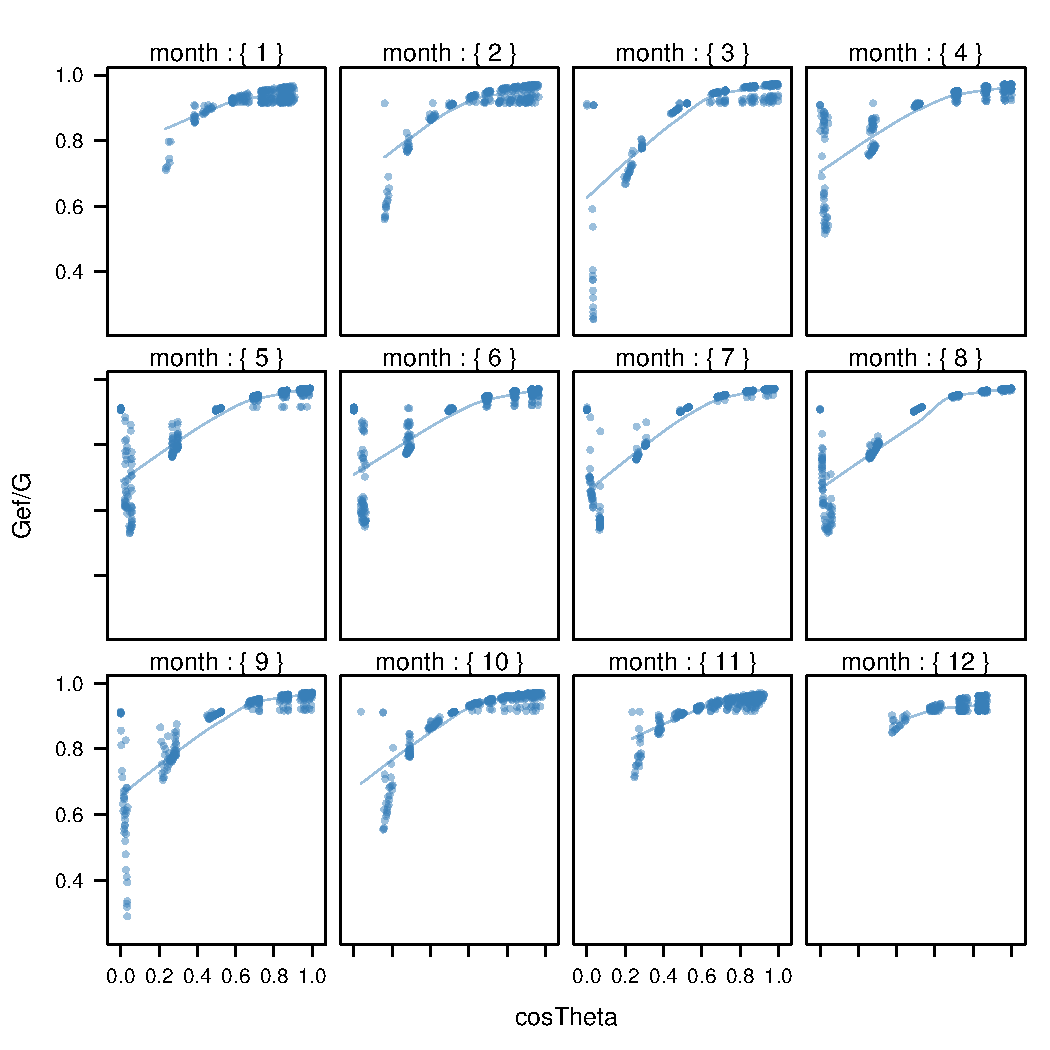
\includegraphics[height=0.4\textheight, keepaspectratio=true]{figs/aoi.pdf}
\par\end{centering}
\caption{Relation between the effective and incident irradiance versus
  the cosine of the angle of incidence for a fixed
  system.\label{fig:GefG0vsTheta}}
\end{figure}

The next lines of code calculate the movement of a N-S horizontal axis
tracker with \emph{backtracking} (\code{modeShd='bt'}) and whose
inclination angle is limited to $\ang{60}$ (\code{betaLim=60}). The
evolution of the inclination angle is displayed in the figure
\ref{fig:Backtracking}. The meaning of the \code{distances} and
\code{struct} arguments will be detailed in the \ref{sec:shadows}
section.

\begin{Schunk}
\begin{Sinput}
> structHoriz = list(L = 4.83)
> distHoriz = data.frame(Lew = structHoriz$L * 4, H = 0)
> gefBT = calcGef(lat = 37.2, dataRad = prom, sample = "10 min", 
     modeTrk = "horiz", modeShd = "bt", betaLim = 60, distances = distHoriz, 
     struct = structHoriz)
\end{Sinput}
\end{Schunk}

\begin{figure}
\begin{centering}
%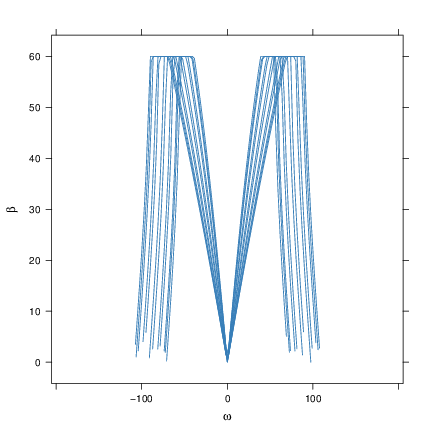
\includegraphics[height=0.4\textheight, keepaspectratio=true]{figs/solaR-032}
\par\end{centering}

\caption{Evolution of the angle of inclination of a NS horizontal axis tracker with \emph{backtracking} and limitation of angle. \label{fig:Backtracking}}

\end{figure}


\section{Productivity of a Grid Connected PV System}
\label{sec:gcpv}

The function \code{fProd}
simulates the performance of a Grid Connected PV (GCPV) system under
certain irradiance and temperature conditions. The system is defined
with a set of parameters: characteristics of the PV
module (\code{module}) and the inverter (\code{inverter}), the electrical arrangement of the PV
generator (\code{generator}) and the losses of the system (\code{effSys}).

For example, the electrical power, voltage and current of a certain PV
system is calculated with:

\begin{Schunk}
\begin{Sinput}
> inclin = data.frame(Gef = c(200, 400, 600, 800, 1000), Ta = 25)
> fProd(inclin)
\end{Sinput}
\begin{Soutput}
   Gef Ta    Tc   Voc   Isc  Vmpp   Impp   Vdc    Idc   Pac   Pdc   EffI
1  200 25 31.75 673.3 10.34 533.1  9.586 533.1  9.586  4212  4737 0.9164
2  400 25 38.50 655.4 20.68 516.3 19.090 516.3 19.090  8275  9137 0.9334
3  600 25 45.25 637.5 31.02 499.6 28.506 499.6 28.506 11972 13202 0.9346
4  800 25 52.00 619.7 41.36 483.0 37.824 483.0 37.824 15323 16936 0.9325
5 1000 25 58.75 601.8 51.70 466.5 47.037 466.5 47.037 18342 20342 0.9293
\end{Soutput}
\end{Schunk}

First, \code{fProd} computes the Maximum Power Point (MPP) of the
generator (\code{Vmpp} and \code{Impp}) at the irradiance and
ambient temperature conditions contained in \code{Inclin}. Next, it
checks that this point is inside the MPP window of the inverter, as
defined by \code{inverter\$Vmin} and \code{inverter\$Vmax}.  If
the MPP value is outside this range, the function assigns the limit
value to the voltage, and calculates the correspondent current value
with a warning.

Anyway, the inverter input voltage and current are  \code{Vdc} e
\code{Idc}. With the next code, the \code{Vdc} value is
set to \code{Vmin} (the minimum value of the MPP window of the
inverter), $\SI{420}{\volt}$,  since \code{Vmpp} is below this value.

\begin{Schunk}
\begin{Sinput}
> inclin = data.frame(Gef = 800, Ta = 30)
> gen1 = list(Nms = 10, Nmp = 11)
> inv1 = list(Ki = c(0.01, 0.025, 0.05), Pinv = 25000, Vmin = 420, 
     Vmax = 750, Gumb = 20)
> prod = fProd(inclin, generator = gen1, inverter = inv1)
> print(prod)
\end{Sinput}
\begin{Soutput}
  Gef Ta Tc   Voc   Isc  Vmpp  Impp Vdc   Idc   Pac   Pdc   EffI
1 800 30 57 505.3 41.36 392.3 37.68 420 33.83 11943 13169 0.9346
\end{Soutput}
\end{Schunk}

For this configuration, the losses due to the voltage limitation are:

\begin{Schunk}
\begin{Sinput}
> with(prod, Vdc * Idc/(Vmpp * Impp))
\end{Sinput}
\begin{Soutput}
[1] 0.961
\end{Soutput}
\end{Schunk}

The function \code{prodGCPV} integrates the calculation procedure of
irradiation, irradiance and simulation of the GCPV system. It
constructs an object of class \code{ProdGCPV}.

The next code computes the productivity of the previous GCPV system
working as fixed, NS horizontal axis tracking and two-axis tracking
systems.  The parameters of the generator, module, inverter and rest
of the system are those by default in \code{prodGCPV}. 

\begin{Schunk}
\begin{Sinput}
> ProdFixed <- prodGCPV(lat = lat, dataRad = prom, keep.night = FALSE)
> Prod2x <- prodGCPV(lat = lat, dataRad = prom, modeTrk = "two", 
     keep.night = FALSE)
> ProdHoriz <- prodGCPV(lat = lat, dataRad = prom, modeTrk = "horiz", 
     keep.night = FALSE)
\end{Sinput}
\end{Schunk}


\subsection[Using mergesolaR]{Using \code{mergesolaR}}
\label{sec:mergesolar}

The \code{mergesolaR} method is designed to merge \emph{daily} time series
of several \pkg{solaR} objects. 

The next example retrieves the daily irradiation of the whole set of
meteorological stations of Madrid (Spain) and use this information to
calculate the productivity of a grid connected PV system with the
\code{lapply} and \code{prodGCPV} functions. The result is a list of
\code{ProdGCPV} objects. In order to prevent from the erroneous
behaviour of some stations, the code includes the use of \code{try}:

\begin{Schunk}
\begin{Sinput}
> EstMadrid <- subset(SIAR, Provincia == "Madrid")
> nEstMadrid <- nrow(EstMadrid)
> namesMadrid <- EstMadrid$Estacion
> prodMadrid <- lapply(1:nEstMadrid, function(x) {
     try(prodGCPV(lat = 41, modeRad = "siar", dataRad = list(prov = 28, 
         est = x, start = "01/01/2009", end = "31/12/2010")))
 })

> names(prodMadrid) <- namesMadrid
> okMadrid <- lapply(prodMadrid, class) != "try-error"
> prodMadrid <- prodMadrid[okMadrid]
> YfMadrid <- do.call(mergesolaR, prodMadrid)

\end{Sinput}
\end{Schunk}

\code{mergesolaR} with a set of \code{ProdGCPV} objects merges
the daily time series of the \code{Yf} variable of each object. The
result is a multivariate \pkg{zoo} object where each column is the
daily productivity with the radiation data of each meteorological
station. It can be displayed (for example) with the
\code{horizonplot} function (figure \ref{fig:horizonMerge}). This
result will be revisited with the \code{Target Diagram} tool (figure
\ref{fig:TargetMerge}). 

\begin{Schunk}
\begin{Sinput}
> horizonplot(YfMadrid - rowMeans(YfMadrid), origin = 0, 
     scales = list(y = list(relation = "same")), colorkey = TRUE))
\end{Sinput}
\end{Schunk}


\begin{figure}
  \centering
%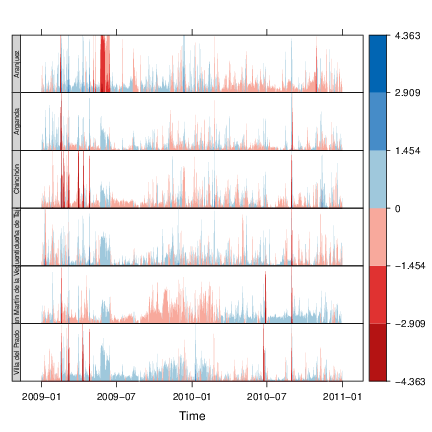
\includegraphics[height=0.4\textheight, keepaspectratio=true]{figs/solaR-041}
\caption{\code{Horizonplot} of the result of a \code{mergesolaR}
    call. Previously, the row mean is substracted from each column in
    order to show the deviation of each meteorological station from
    the daily mean of the set.}
  \label{fig:horizonMerge}
\end{figure}





\subsection{Shadows}
\label{sec:shadows}

The shadows on PV generators alter the performance of the PV
generators and reduce their productivity \cite{Perpinan2008}.  This
package includes functions for the estimation of mutual shadows
between generators belonging to the same system. \code{fSombra2X},
\code{fSombraHoriz}, \code{fSombraEst}, calculate the shadows in
two-axis, horizontal axis and fixed systems, respectively.  The
function \code{fSombra6} is indicated for groups of two-axis
trackers.  Finally, \code{fSombra} is a wrapper to the previous
functions. These functions are integrated in \code{calcShd},
\code{calcGef} and \code{prodGCPV}, as these examples show.

First, the dimensions of the support structures (\code{struct}) and
the distances between them (\code{distances}) have to be defined. 
With a two-axis tracking system:
\begin{Schunk}
\begin{Sinput}
> struct2x = list(W = 23.11, L = 9.8, Nrow = 2, Ncol = 8)
> dist2x = data.frame(Lew = 40, Lns = 30, H = 0)
> prod2xShd <- prodGCPV(lat = lat, dataRad = prom, modeTrk = "two", 
     modeShd = "area", struct = struct2x, distances = dist2x)
\end{Sinput}
\end{Schunk}

Then, a N-S horizontal axis tracking system without backtracking, 
\begin{Schunk}
\begin{Sinput}
> structHoriz = list(L = 4.83)
> distHoriz = data.frame(Lew = structHoriz$L * 4, H = 0) 
> prodHorizShd <- prodGCPV(lat = lat, dataRad = prom, sample = "10 min", 
     modeTrk = "horiz", modeShd = "area", betaLim = 60, distances = distHoriz, 
     struct = structHoriz)
\end{Sinput}
\end{Schunk}

and a N-S horizontal axis tracking system with backtracking, 
\begin{Schunk}
\begin{Sinput}
> prodHorizBT <- prodGCPV(lat = lat, dataRad = prom, sample = "10 min", 
     modeTrk = "horiz", modeShd = "bt", betaLim = 60, distances = distHoriz, 
     struct = structHoriz)
\end{Sinput}
\end{Schunk}

Finally, the \emph{yearly} performance of these systems is compared
with the method \code{compare} (fig. \ref{fig:compare}):
\begin{Schunk}
\begin{Sinput}
> comp <- compare(ProdFixed, Prod2x, ProdHoriz, prod2xShd, 
     prodHorizShd, prodHorizBT)
> head(comp)
\end{Sinput}
\begin{Soutput}
  values  ind      name
1   1836  G0d ProdFixed
2   1969 Gefd ProdFixed
3   1506   Yf ProdFixed
4   1836  G0d    Prod2x
5   2961 Gefd    Prod2x
6   2235   Yf    Prod2x
\end{Soutput}
\end{Schunk}

The methods \code{losses} and \code{compareLosses} calculate and
compare their \emph{yearly} losses, respectively (fig. \ref{fig:compareLosses}):

\begin{Schunk}
\begin{Sinput}
> compL <- compareLosses(ProdFixed, Prod2x, ProdHoriz, prod2xShd, 
     prodHorizShd, prodHorizBT)
> head(compL)
\end{Sinput}
\begin{Soutput}
         id  values      name
1   Shadows 0.00000 ProdFixed
2       AoI 0.05894 ProdFixed
3 Generator 0.08392 ProdFixed
4        DC 0.07441 ProdFixed
5  Inverter 0.07038 ProdFixed
6        AC 0.02973 ProdFixed
\end{Soutput}
\end{Schunk}

 
\begin{figure}
  \centering
%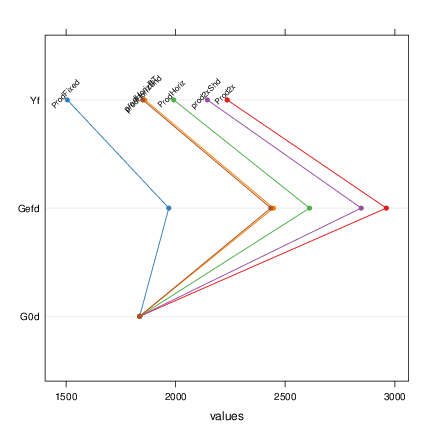
\includegraphics[height=0.4\textheight, keepaspectratio=true]{figs/solaR-048}
  \caption{Comparison of several \code{ProdGCPV} objects.}
  \label{fig:compare}
\end{figure}

\begin{figure}
  \centering
%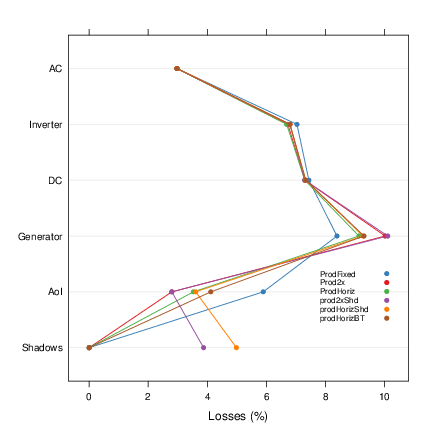
\includegraphics[height=0.4\textheight, keepaspectratio=true]{figs/solaR-049}
  \caption{Comparison of the losses of several \code{ProdGCPV} objects.}
  \label{fig:compareLosses}
\end{figure}


\subsection{Position of trackers in a PV plant}
\label{sec:trackers}
One of the tasks of the design of a PV tracking system is to place the
set of trackers. This task must cope with the compromise of minimizing
the losses due to mutual shadows while requiring the minimum land
area.

The area of the PV generator and the total land requirement are
commonly related with the Ground Coverage Ratio (GCR). This ratio
quantifies the percentage of land being effectively occupied by the
system. In order to focus on the land area required, the inverse of
this ratio, the Ground Requirement Ratio (GRR), is preferable. The GRR
is the ratio between the ground area required for installing the whole
set of trackers and the generator area.

A suitable approach to the problem is to simulate the planned system
for a set of distances between the trackers of the plant. Without any
additional constraint, the optimum design may be the one which
achieves the highest productivity with the lowest ground requirement
ratio. 

However, it should be noted that this approach to the problem is not
complete since the land requirements and the costs of wiring and
equipments should be included as additional constraints
\cite{Perpinan2011b}.

The function \code{optimShd} computes the productivity for a set of
combinations of distances between the elements of the plant
\cite{Perpinan2008}. The designer should adopt the decision from
these results with the adequate economical translations.

For example, let's design a PV plant with a grid of trackers of 2 rows
and 8 columns using a two-axis tracker whose dimensions are
$\SI{23.11}{\meter}$ width and $\SI{9.8}{\meter}$ height.

\begin{Schunk}
\begin{Sinput}
> struct2x = list(W = 23.11, L = 9.8, Nrow = 2, Ncol = 8)
\end{Sinput}
\end{Schunk}

The separations between trackers range from $\SI{30}{\meter}$ and
$\SI{50}{\meter}$ for the East-West direction and from $\SI{20}{\meter}$
and $\SI{50}{\meter}$ for the North-South direction.

\begin{Schunk}
\begin{Sinput}
> dist2x = list(Lew = c(30, 50), Lns = c(20, 50))
\end{Sinput}
\end{Schunk}

\code{optimShd} constructs a sequence from the minimum to the
maximum value of \code{distances}, with \code{res} as the
increment, in meters, of the sequence. In this example,
\code{res=5}.

\begin{Schunk}
\begin{Sinput}
> ShdM2x <- optimShd(lat = lat, dataRad = prom, modeTrk = "two", 
     modeShd = c("area", "prom"), distances = dist2x, struct = struct2x, 
     res = 5, prog = FALSE)

> shadeplot(ShdM2x)
\end{Sinput}
\end{Schunk}

Besides, the \code{Shade} object includes the local fitting of the
sequence of \code{Yf} and \code{FS} values (slots named
\code{Yf.loess} and \code{FS.loess}). The \code{predict} method is
used with these \code{loess} slots inside the \code{shadeplot} method
of the \code{Shade} class (figure \ref{fig:optim2x}).


\begin{figure}
\centering
%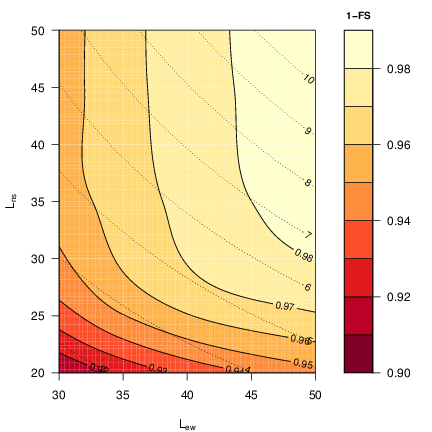
\includegraphics[height=0.4\textheight, keepaspectratio=true]{figs/solaR-058}

\caption{Mutual shadows in a two-axis tracking PV system for a
  combination of separations between trackers.\label{fig:optim2x}}

\end{figure}



\section{PV pumping systems}
\label{sec:pumping}

\subsection{Simulation of centrifugal pumps}

The first step for the simulation of the performance of a PV pumping
system (PVPS) is the characterization of the pump under the
supposition of constant manometric height
\cite{Abella.Lorenzo.ea2003}. The function \code{fPump} computes the
performance of the different parts of a centrifugal pump fed by a
frequency converter following the affinity laws.

For example, the performance of the SP8A44 pump
\footnote{\url{http://net.grundfos.com/Appl/WebCAPS/InitCtrl?mode=1}},
whose information is available in the dataset \code{pumpCoef}, working
with $H=\SI{40}{m}$ is simulated with:

\begin{Schunk}
\begin{Sinput}
> data("pumpCoef")
> CoefSP8A44 <- subset(pumpCoef, Qn == 8 & stages == 44)
> fSP8A44 <- fPump(pump = CoefSP8A44, H = 40)
\end{Sinput}
\end{Schunk}

The result of \code{fPump} is a set of functions which relate the
electrical power and the flow, hydraulical and mechanical power, and
frequency.  These functions allow the calculation of the performance
for any electrical power inside the range of the pump (figure
\ref{fig:EficienciaMotobomba}):

\begin{Schunk}
\begin{Sinput}
> SP8A44 = with(fSP8A44, {
     Pac = seq(lim[1], lim[2], by = 100)
     Pb = fPb(Pac)
     etam = Pb/Pac
     Ph = fPh(Pac)
     etab = Ph/Pb
     f = fFreq(Pac)
     Q = fQ(Pac)
     result = data.frame(Q, Pac, Pb, Ph, etam, etab, f)
 })
> SP8A44$etamb = with(SP8A44, etab * etam) 

> lab = c(expression(eta[motor]), expression(eta[pump]), expression(eta[mp]))
> p <- xyplot(etam + etab + etamb ~ Pac, data = SP8A44, type = "l", 
     ylab = "Efficiency")
> p + glayer(panel.text(x[1], y[1], lab[group.number], pos = 3))

\end{Sinput}
\end{Schunk}


\begin{figure}
\centering
%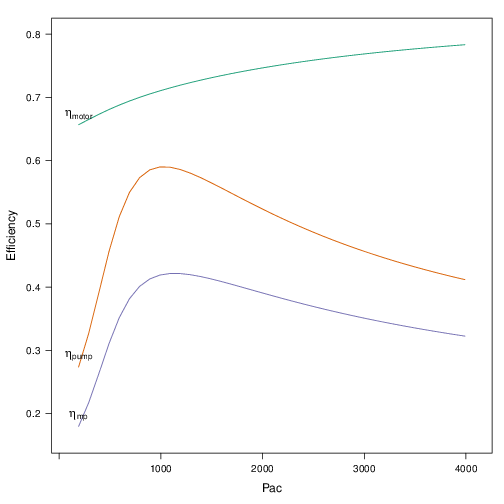
\includegraphics[height=0.4\textheight, keepaspectratio=true]{figs/efficiencyPVPS}

\caption{Efficiency of the motor and pump for several values of
  electrical power of a SP8A44 pump with
  $H=\SI{40}{m}$\label{fig:EficienciaMotobomba}}

\end{figure}

The performance of a PVPS follows the same procedure as the one
described for the GCPV systems.  The function \code{prodPVPS} is the
equivalent to the function \code{prodGCPV}.  The inputs are very
similar between them, although there are some changes due to the
different composition of the system. This function does not allow for
the calculation of shadows.

\subsection{Nomograms of PVPS}

The international standard IEC 61725 is of common usage in public
licitations of PVPS.  This standard proposes a equation of the
irradiance profile with several parameters such as the length of the
day, the daily irradiation and the maximum value of the irradiance.
With this profile, the performance of a PVPS can be calculated for
several manometric heights and nominal PV power values. A nomogram can
display the set of combinations.  This graphical tool can help to
choose the best combination of pump and PV generator for certain
conditions of irradiation and height \cite{Abella.Lorenzo.ea2003}.

This kind of graphics is provided by the function
\code{NmgPVPS}. For example, the figure \ref{fig:Nomograma} is a
nomogram for the SP8A44 pump working in a range of heights from 50 to
80 meters, with different PV generators. The peculiar shape of the
curve of 50 meters shows that this pump does not work correctly with
this height.

\begin{Schunk}
\begin{Sinput}
> Pg = seq(3000, 5500, by = 500)
> H = seq(50, 80, by = 5)
> NmgSP8A44 <- NmgPVPS(pump = CoefSP8A44, Pg = Pg, H = H, Gd = 6000, 
     title = "Selection of Pumps")
\end{Sinput}
\end{Schunk}

\begin{figure}
\begin{centering}
%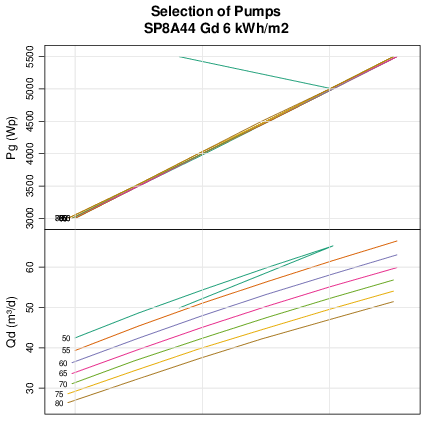
\includegraphics[height=0.4\textheight, keepaspectratio=true]{figs/solaR-063}
\par\end{centering}

\caption{Nomogram for the SP8A44 pump working in a range of heights
  from 50 to 80 meters, with different PV
  generators.\label{fig:Nomograma}}

\end{figure}


\section{Spatial calculations}
\label{sec:spatial}

\pkg{solaR} is designed for time series associated to a
location defined by the latitude and longitude values, and the
temperature and irradiation conditions. However, \pkg{solaR} can also be
easily combined with spatial packages: for example with \pkg{raster}
\cite{Hijmans.vanEtten2011} in \cite{Ummel2011} o with geostatistics
methods in \cite{Perpinan2011d}.

\subsection[sp]{\pkg{solaR} and \pkg{sp}}
\label{sec:sp}


As an example of the interaction of \pkg{sp} and \pkg{solaR}, let's
draw a map of the extraterrestial irradiance. First, the mean solar time for a range of
longitudes with \code{local2Solar} is calculated with:

\begin{Schunk}
\begin{Sinput}
> hh <- as.POSIXct('2011-05-01 11:00:00', tz='CET')
> latitude <- seq(70, -70, -1)
> longitude <- seq(-180, 180, 1)
> horaLong <- local2Solar(hh, longitude)
\end{Sinput}
\end{Schunk}

Then, the irradiance for the window defined by \code{latitude} and
\code{longitude} is calculated with \code{calcSol}. The zero value is
assigned to the \code{NA} elements in order to get them black coloured
in the map.

\begin{Schunk}
\begin{Sinput}
> solList <- lapply(latitude, calcSol, BTi = horaLong)
> Bo0List <- lapply(solList, function(x) as.data.frameI(x)$Bo0) 
> Bo0 <- do.call('c', Bo0List)
> Bo0[is.na(Bo0)] <- 0
\end{Sinput}
\end{Schunk}


The \code{data.frame} is now converted to an
\code{SpatialPixelsDataFrame}. The result is displayed in the figure \ref{fig:Bo0Map}.
\begin{Schunk}
\begin{Sinput}
> Bo0DF <- expand.grid(lon = longitude, lat = latitude)
> Bo0DF$Bo0 <- c(Bo0)
> proj <- CRS('+proj=latlon +ellps=WGS84') 
> Bo0SP <- SpatialPixelsDataFrame(points = Bo0DF[,1:2],
      data=Bo0DF["Bo0"], proj4string = proj)

> paleta=colorRampPalette(rev(brewer.pal('Greys', n=9)))
> p <- spplot(Bo0SP, scales = list(draw = TRUE), col.regions = paleta,
      cuts = 50)
> world <- map("world", plot = FALSE)
> world_sp <- map2SpatialLines(world, proj4string = proj)
> p2 <- p+layer(sp.lines(world_sp, lwd = 0.5))
\end{Sinput}
\end{Schunk}

\begin{figure}
  \centering
%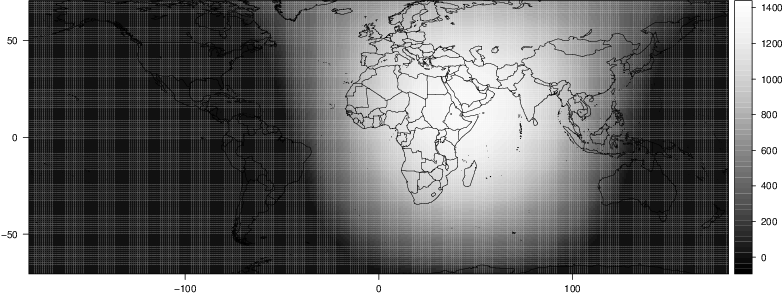
\includegraphics[height = 0.4\textheight, keepaspectratio = true]{figs/bo0_crop.pdf}
  \caption{Extraterrestial irradiance map}
  \label{fig:Bo0Map}
\end{figure}

\subsection[raster]{\pkg{solaR} and \pkg{raster}}
\label{sec:raster}


As an example of the interaction of \pkg{raster} and \pkg{solaR},
several files with monthly averages of global solar radiation over the
Iberian
Peninsula\footnote{\url{http://www.box.net/shared/rl51y1t9sldxk54ogd44}}
are read with \pkg{raster} and transformed with \pkg{solaR}. This
information is provided by the Satellite Application Facility on
Climate Monitoring (CMSAF)\footnote{\url{http://www.cmsaf.eu/}}. CMSAF
generates, archives and distributes widely recognised high-quality
satellite-derived products and services relevant for climate
monitoring in operational mode. The data is freely accesible here
after a registration process.


\begin{Schunk}
\begin{Sinput}
> library("raster")
> old <- setwd('CMSAF') ##folder where the files are stored
> listFich <- dir(pattern = '2008')
> stackSIS <- stack(listFich)
> stackSIS <- stackSIS*24 ##from irradiance (W/m2) to irradiation Wh/m2
> setwd(old)
\end{Sinput}
\end{Schunk}

The yearly effective irradiance on an inclined plane can be calculated
with \code{calcGef} (section \ref{sec:effective}). The next function uses \code{calcGef} to provide
yearly values (\code{as.data.frameY}) of effective global, diffuse and
direct irradiation:

\begin{Schunk}
\begin{Sinput}
> foo <- function(x, ...){
               gef <- calcGef(lat = x[1], dataRad = list(G0dm = x[2:13]))
               result <- as.data.frameY(gef)[c('Gefd', 'Befd', 'Defd')]
               as.numeric(result)
  }
\end{Sinput}
\end{Schunk}


The function \code{calc} from \pkg{raster} applies this function to each
cell of the \code{raster}:

\begin{Schunk}
\begin{Sinput}
> latLayer <- init(SISmm, v = 'y')
> gefS <- calc(stack(latLayer, SISmm), foo,
             filename = 'CMSAF/gefCMSAF',
             overwrite = TRUE)
> layerNames(gefS) <- c('Gefd', 'Befd', 'Defd')
\end{Sinput}
\end{Schunk}

The figure \ref{fig:CMSAF} displays the results for the global
effective irradiation using the
\code{levelplot} method included in the \pkg{rasterVis} package, with the administrative borders
overlaid\footnote{Available at
  \url{http://biogeo.ucdavis.edu/data/diva/adm/ESP_adm.zip}} with the
\code{layer} mechanism of the \pkg{latticeExtra} package:

\begin{Schunk}
\begin{Sinput}
> library("maptools")
> library("rasterVis")
> proj <- CRS(projection(SISmm))
> mapaSHP <- readShapeLines('ESP_adm2.shp', proj4string = proj)
> levelplot(gefS, layers = 'Gefd') + layer(sp.lines(mapaSHP, lwd = 0.7))
\end{Sinput}
\end{Schunk}

\begin{figure}
  \centering
%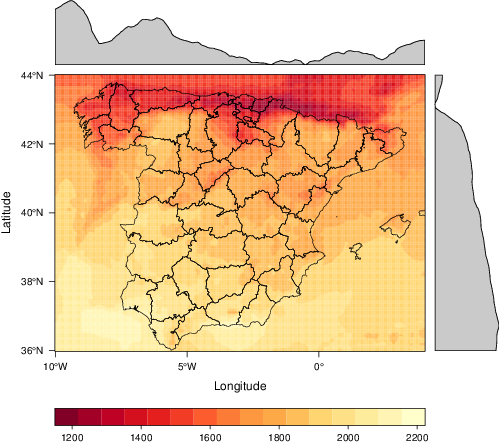
\includegraphics[height=0.4\textheight, keepaspectratio=true]{figs/CMSAF_Gef-crop}
  \caption{Global effective irradiation in Spain calculated from the
    CMSAF irradiation data. \label{fig:CMSAF}}
\end{figure}


\section{Target Diagram}
\label{sec:target_diagram}

In a PV plant, the individual systems are theoretically identical and
their performance along the time should be the same. Due to their
practical differences --power tolerance, dispersion losses, dust--,
the individual performance of each system will deviate from the
average behaviour. However, when a system is performing correctly,
these deviations are constrained inside a range and should not be
regarded as a sign of malfunctioning.

If these common deviations are assumed as a random process, a
statistical analysis of the performance of the whole set of systems
can identify a faulty system as the one that departs significantly
from the mean behaviour \cite{Perpinan2009}.

The functions \code{analyzeData} and \code{TargetDiagram} compare the
daily performance of each system with a reference (for example, the
median of the whole set) during a time period of N days preceding the
current day. They calculate a set of statistics of the performance of
the PV plant as a whole, and another set of the comparison with the
reference. 

This statistical analysis can be summarised with a graphical tool
named "Target Diagram", which plots together the root mean square
difference, the average difference and the standard deviation of the
difference. Besides, this diagram includes the sign of the difference
of the standard deviations of the system and the reference
\cite{Jolliff.Kindle.ea2009,Taylor2000}.

The example of the figure \ref{fig:TargetDiagram} uses a dataset of
productivity from a PV plant composed of 22 systems
(\code{data("prodEx")}) showing that the system no.20 is not
working correctly during these periods.

\begin{Schunk}
\begin{Sinput}
> data("prodEx")
> ndays = c(5, 10, 15, 20)
> palette = brewer.pal(n = length(ndays), name = "Set1")
> TDColor <- TargetDiagram(prodEx, end = day, 
      ndays = ndays, 
      color = palette)
\end{Sinput}
\end{Schunk}

\begin{figure}
  \centering
%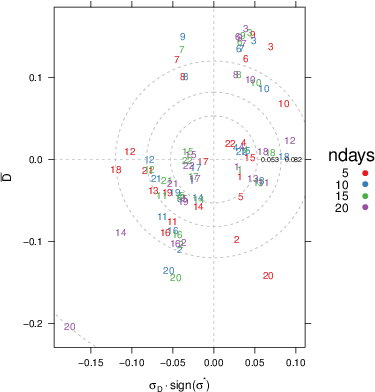
\includegraphics[height=0.4\textheight, keepaspectratio=true]{figs/TDprod_crop}
  \caption{``Target Diagram'' of the statistical analysis of a set of 22 systems during various time periods.}
  \label{fig:TargetDiagram}
\end{figure}

The figure \ref{fig:horizonMerge} displayed the result of an example
with \code{mergesolaR} and the SIAR network. The function
\code{TargetDiagram} is an alternative tool to show the behaviour of
the set of meteorological stations (figure
\ref{fig:TargetMerge}). Once again, the behaviour of the Aranjuez
station is consistently different from the rest of the stations of Madrid during
these time intervals.

\begin{Schunk}
\begin{Sinput}
> TDMadrid <- TargetDiagram(YfMadrid, 
     end = as.POSIXct("2010-12-31"), 
     ndays = c(10, 20, 30, 40, 50, 60), 
     cex = 0.7)
\end{Sinput}
\end{Schunk}

\begin{figure}
  \centering
%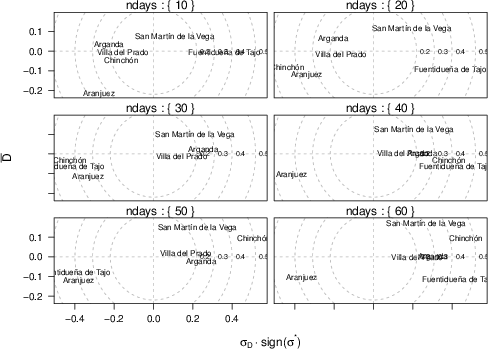
\includegraphics[height=0.4\textheight, keepaspectratio=true]{figs/TDMadrid_crop}
  \caption{Target Diagram of the result of the mergesolaR example}
  \label{fig:TargetMerge}
\end{figure}

\bibliographystyle{plain}
\bibliography{solaR}

\end{document}
